% Options for packages loaded elsewhere
\PassOptionsToPackage{unicode}{hyperref}
\PassOptionsToPackage{hyphens}{url}
%
\documentclass[
]{book}
\usepackage{lmodern}
\usepackage{amsmath}
\usepackage{ifxetex,ifluatex}
\ifnum 0\ifxetex 1\fi\ifluatex 1\fi=0 % if pdftex
  \usepackage[T1]{fontenc}
  \usepackage[utf8]{inputenc}
  \usepackage{textcomp} % provide euro and other symbols
  \usepackage{amssymb}
\else % if luatex or xetex
  \usepackage{unicode-math}
  \defaultfontfeatures{Scale=MatchLowercase}
  \defaultfontfeatures[\rmfamily]{Ligatures=TeX,Scale=1}
\fi
% Use upquote if available, for straight quotes in verbatim environments
\IfFileExists{upquote.sty}{\usepackage{upquote}}{}
\IfFileExists{microtype.sty}{% use microtype if available
  \usepackage[]{microtype}
  \UseMicrotypeSet[protrusion]{basicmath} % disable protrusion for tt fonts
}{}
\makeatletter
\@ifundefined{KOMAClassName}{% if non-KOMA class
  \IfFileExists{parskip.sty}{%
    \usepackage{parskip}
  }{% else
    \setlength{\parindent}{0pt}
    \setlength{\parskip}{6pt plus 2pt minus 1pt}}
}{% if KOMA class
  \KOMAoptions{parskip=half}}
\makeatother
\usepackage{xcolor}
\IfFileExists{xurl.sty}{\usepackage{xurl}}{} % add URL line breaks if available
\IfFileExists{bookmark.sty}{\usepackage{bookmark}}{\usepackage{hyperref}}
\hypersetup{
  pdftitle={GIS and Spatial Analysis for Conservation Biology Using R},
  pdfauthor={Dr.~Yolanda Wiersma, Memorial University},
  hidelinks,
  pdfcreator={LaTeX via pandoc}}
\urlstyle{same} % disable monospaced font for URLs
\usepackage{color}
\usepackage{fancyvrb}
\newcommand{\VerbBar}{|}
\newcommand{\VERB}{\Verb[commandchars=\\\{\}]}
\DefineVerbatimEnvironment{Highlighting}{Verbatim}{commandchars=\\\{\}}
% Add ',fontsize=\small' for more characters per line
\usepackage{framed}
\definecolor{shadecolor}{RGB}{248,248,248}
\newenvironment{Shaded}{\begin{snugshade}}{\end{snugshade}}
\newcommand{\AlertTok}[1]{\textcolor[rgb]{0.94,0.16,0.16}{#1}}
\newcommand{\AnnotationTok}[1]{\textcolor[rgb]{0.56,0.35,0.01}{\textbf{\textit{#1}}}}
\newcommand{\AttributeTok}[1]{\textcolor[rgb]{0.77,0.63,0.00}{#1}}
\newcommand{\BaseNTok}[1]{\textcolor[rgb]{0.00,0.00,0.81}{#1}}
\newcommand{\BuiltInTok}[1]{#1}
\newcommand{\CharTok}[1]{\textcolor[rgb]{0.31,0.60,0.02}{#1}}
\newcommand{\CommentTok}[1]{\textcolor[rgb]{0.56,0.35,0.01}{\textit{#1}}}
\newcommand{\CommentVarTok}[1]{\textcolor[rgb]{0.56,0.35,0.01}{\textbf{\textit{#1}}}}
\newcommand{\ConstantTok}[1]{\textcolor[rgb]{0.00,0.00,0.00}{#1}}
\newcommand{\ControlFlowTok}[1]{\textcolor[rgb]{0.13,0.29,0.53}{\textbf{#1}}}
\newcommand{\DataTypeTok}[1]{\textcolor[rgb]{0.13,0.29,0.53}{#1}}
\newcommand{\DecValTok}[1]{\textcolor[rgb]{0.00,0.00,0.81}{#1}}
\newcommand{\DocumentationTok}[1]{\textcolor[rgb]{0.56,0.35,0.01}{\textbf{\textit{#1}}}}
\newcommand{\ErrorTok}[1]{\textcolor[rgb]{0.64,0.00,0.00}{\textbf{#1}}}
\newcommand{\ExtensionTok}[1]{#1}
\newcommand{\FloatTok}[1]{\textcolor[rgb]{0.00,0.00,0.81}{#1}}
\newcommand{\FunctionTok}[1]{\textcolor[rgb]{0.00,0.00,0.00}{#1}}
\newcommand{\ImportTok}[1]{#1}
\newcommand{\InformationTok}[1]{\textcolor[rgb]{0.56,0.35,0.01}{\textbf{\textit{#1}}}}
\newcommand{\KeywordTok}[1]{\textcolor[rgb]{0.13,0.29,0.53}{\textbf{#1}}}
\newcommand{\NormalTok}[1]{#1}
\newcommand{\OperatorTok}[1]{\textcolor[rgb]{0.81,0.36,0.00}{\textbf{#1}}}
\newcommand{\OtherTok}[1]{\textcolor[rgb]{0.56,0.35,0.01}{#1}}
\newcommand{\PreprocessorTok}[1]{\textcolor[rgb]{0.56,0.35,0.01}{\textit{#1}}}
\newcommand{\RegionMarkerTok}[1]{#1}
\newcommand{\SpecialCharTok}[1]{\textcolor[rgb]{0.00,0.00,0.00}{#1}}
\newcommand{\SpecialStringTok}[1]{\textcolor[rgb]{0.31,0.60,0.02}{#1}}
\newcommand{\StringTok}[1]{\textcolor[rgb]{0.31,0.60,0.02}{#1}}
\newcommand{\VariableTok}[1]{\textcolor[rgb]{0.00,0.00,0.00}{#1}}
\newcommand{\VerbatimStringTok}[1]{\textcolor[rgb]{0.31,0.60,0.02}{#1}}
\newcommand{\WarningTok}[1]{\textcolor[rgb]{0.56,0.35,0.01}{\textbf{\textit{#1}}}}
\usepackage{longtable,booktabs}
\usepackage{calc} % for calculating minipage widths
% Correct order of tables after \paragraph or \subparagraph
\usepackage{etoolbox}
\makeatletter
\patchcmd\longtable{\par}{\if@noskipsec\mbox{}\fi\par}{}{}
\makeatother
% Allow footnotes in longtable head/foot
\IfFileExists{footnotehyper.sty}{\usepackage{footnotehyper}}{\usepackage{footnote}}
\makesavenoteenv{longtable}
\usepackage{graphicx}
\makeatletter
\def\maxwidth{\ifdim\Gin@nat@width>\linewidth\linewidth\else\Gin@nat@width\fi}
\def\maxheight{\ifdim\Gin@nat@height>\textheight\textheight\else\Gin@nat@height\fi}
\makeatother
% Scale images if necessary, so that they will not overflow the page
% margins by default, and it is still possible to overwrite the defaults
% using explicit options in \includegraphics[width, height, ...]{}
\setkeys{Gin}{width=\maxwidth,height=\maxheight,keepaspectratio}
% Set default figure placement to htbp
\makeatletter
\def\fps@figure{htbp}
\makeatother
\setlength{\emergencystretch}{3em} % prevent overfull lines
\providecommand{\tightlist}{%
  \setlength{\itemsep}{0pt}\setlength{\parskip}{0pt}}
\setcounter{secnumdepth}{5}
\usepackage{booktabs}
\ifluatex
  \usepackage{selnolig}  % disable illegal ligatures
\fi
\usepackage[]{natbib}
\bibliographystyle{apalike}

\title{GIS and Spatial Analysis for Conservation Biology Using R}
\author{Dr.~Yolanda Wiersma, Memorial University}
\date{2021-01-22}

\begin{document}
\maketitle

{
\setcounter{tocdepth}{1}
\tableofcontents
}
\hypertarget{intro}{%
\chapter{Introduction}\label{intro}}

Many biology-relevant skills are now performed using computers: statistical analyses, mathematical modelling, managing and reformatting data, visualizing data, identifying genes from DNA sequences, constructing 3D models of proteins, and making phylogenies. Quantitative skills and best practices in data science are now being incorporated throughout the biology major.

In Ecology and Conservation Biology, it is common for researchers to use spatial mapping tools such as Geographic Information Systems (GIS). The most common GIS software is the ESRI suite of products (ArcGIS, ArcPro, ArcONline). This software is expensive, and can be time consuming to learn. While R is not a GIS SYSTEM, it has the capabilities to create maps and to do many of tye types of spatial analyses that ecologists would use a GIS for. R can also be time-consuming to learn, but because R is free, we feel it will have advantages for students in that they will always be able to access it. Many ENGOs may wish to create maps and do spatial analysis, but lack the financial resources to purchase GIS. Thus, graduates who can do analysis in R will be well-positioned to contribute usefully in many conservation sectors.

\hypertarget{howto}{%
\chapter{How to use this manual}\label{howto}}

This manual has been developed specifically for Biology students. We are increasing the focus on quantitative skills in our Biology curriculum, in response to changing demands and emphasis within the field of biology itself. In 2020, we introduce first year biology (BIOL 1001/1002) students to R software and basic statistical concepts. Other courses (BIOL 2600 - Principles of Ecology, BIOL 3295 - Population and Evolutionary Ecology and BIOL 4607 - Models in Biology) all incorporate R tools in their labs. This course will teach you some R tools relevant to spatial analysis for conservation biology.

If you are not familiar with R, it is recommended that you read through the MUN Biology R Manual, which is available online \href{https://ahurford.github.io/quant-guide-all-courses/}{here}, paying special attention to chapters 2-7.

While working through the manual, we recommend that you set up your computer screen so that you can see your browser and the R Studio software at the same time. You can experiment with re-sizing windows and if you have two monitors, that will be really handy. Or, if you have access to a laptop and a tablet, we recommend using RStudio on your laptop and opening the manual in the browser on your tablet so that you can move between the two easily.

\hypertarget{whatIs}{%
\chapter{What is GIS?}\label{whatIs}}

GIS (Geographic Information Systems) is defined as ``A geographic information system (GIS) is a framework for gathering, managing, and analyzing data. Rooted in the science of geography, GIS integrates many types of data. It analyzes spatial location and organizes layers of information into visualizations using maps and 3D scenes. With this unique capability, GIS reveals deeper insights into data, such as patterns, relationships, and situations---helping users make smarter decisions.'' (ESRI.com)

Many people think GIS is simply software for making maps. While you can make maps with a GIS, that is not the real purpose (to make really great maps, one would use cartographic software). A GIS is a spatial database. It allows you to store, organize, query, and analyze data - but not just any data - data in a GIS have specific spatial reference. Thus, the spatial location of data is linked to the attributes, and data can be analyzed based on both the spatial location AND the attributes of the data themselves.

GIS is very powerful software and is used in many sectors of society. The biggest users of GIS software are in marketing, urban/municipal planning, and the military. Conservation and ecology researchers are actually in a small minority of GIS users.

This manual will introduce some of the commont things that conservation biologists will want to do with spatial data. These include:

\begin{enumerate}
\def\labelenumi{\arabic{enumi}.}
\tightlist
\item
  visualizing data in a map
\item
  using sampling points to sample map data
\item
  using polygons to sample map data
\end{enumerate}

As well, this manual will introduce some of the common issues and challenges when dealing with spatial data, including challenges with projections, map symbology, scale issues, and data organization.

\hypertarget{types-of-gis-data}{%
\section{Types of GIS Data}\label{types-of-gis-data}}

GIS data are divided into two categories, raster data and vector data. Another important component of GIS data is the metadata.

\hypertarget{raster-data}{%
\section{Raster Data}\label{raster-data}}

Raster data represent the spatial data as a map made of pixels (sometimes called a ``raster''). Each pixel has a unique value, in addition to a x, y coordinate. Raster data may be continuous, and represnet the actual value of the feature in the real world (e.g., soil pH) or raster data may be categorical, with numbers standing in for categorical data (e.g., 3 = decidous forest). In this case, the metadata should include a description of what the pixel data represent.

\hypertarget{vector-data}{%
\section{Vector Data}\label{vector-data}}

Vector data represent the spatial data as either points, lines or polygons. Each feature in the dataset has georeferenced data (its locatoin along an x, y coordinate system) as well as attribute data. The attribute data can have many files. For example, a polygon feature representing protected areas might have fields for the name of the protected area, the year it was established, its size, the type of protected area (e.g., national, provincial or state park), and other data. Each line (or record) in the attribute data file is linked to a single feature in the data set.

There are no rules for what kind of data must be represented as either points, lines or polygons, however there are some standard (and farily obvious) practices. Features that are generally linear in the real world (even if they are not perfectly one-dimensional), such as roads, rivers, and railways, are usually represented by lines. Sample points and single entities (e.g., single trees) are reprsented as points. Features that have 2 dimensions, such as parcels of land, are represented as polygons. Sometimes a feature may be shown as a point at one spatial scale (e.g., at the scale of a continent, cities are shown as points) but as polygons at another spatial scale (e.g., if we zoom in on the Northeast Avalon, we may want to show the municipal boundaries of the various cities and towns as polygons).

\hypertarget{metadata}{%
\section{Metadata}\label{metadata}}

Metadata is ``data about the data''. Metadata is a very important component of good data practice and is discusssed in chapter 10 of the MUN Biology R manual. If you are unfamilair with the concept of metadata, you can review it \href{https://ahurford.github.io/quant-guide-all-courses/data.html}{here}. With GIS data, the metadata are especially important, as they contain information about the coordinate reference system, or CRS (see chapter \ref{projections}), as well as the attribute data, along with information about how and when the data were created.

\hypertarget{vector}{%
\chapter{Reading in Vector Data}\label{vector}}

We will use the R package \texttt{sf} for handling vector data. You will have to download and install this package from the CRAN repository (review section \href{https://ahurford.github.io/quant-guide-all-courses/rintro.html\#r-packages}{4.10} of the MUN Biology R manual if need a reminder of how to do this).

\begin{Shaded}
\begin{Highlighting}[]
\FunctionTok{library}\NormalTok{(sf)}
\end{Highlighting}
\end{Shaded}

To plot the data (i.e., make a map) we will also need the package \texttt{ggplot2}, so make sure to load and install that as well.

\begin{Shaded}
\begin{Highlighting}[]
\FunctionTok{library}\NormalTok{(ggplot2)}
\end{Highlighting}
\end{Shaded}

Download the folder ``HARV'' to your working directory. If you do not remember how to check, and set your working directory, review section \href{https://ahurford.github.io/quant-guide-all-courses/rintro.html\#working-directory}{4.2}. This folder contains data from the Harvard Research Forest. The vector data include a point file that represents sampling points, a line file that is the boundary of the resarch forest, and two polygon files that show the boundary of the research forest and the soil regions.

We read these files in in a similar way as you read in a file like a csv file, but instead of using \texttt{read.csv} we use \texttt{st\_read()}

Read in the boundary shapefile (recognizable by the .shp extension) for the Harvard forest

\begin{Shaded}
\begin{Highlighting}[]
\NormalTok{HARV\_boundary }\OtherTok{\textless{}{-}} \FunctionTok{st\_read}\NormalTok{(}\StringTok{"HARV/harv\_boundary.shp"}\NormalTok{)}
\end{Highlighting}
\end{Shaded}

\begin{verbatim}
## Reading layer `harv_boundary' from data source `C:\Users\ywiersma\Documents\BIOL4651\GIS_R_manual\ConsBiol_SpatialAnalysis\HARV\harv_boundary.shp' using driver `ESRI Shapefile'
## Simple feature collection with 1 feature and 8 fields
## geometry type:  MULTIPOLYGON
## dimension:      XY
## bbox:           xmin: 730167.7 ymin: 4712097 xmax: 732532.1 ymax: 4714961
## projected CRS:  WGS 84 / UTM zone 18N
\end{verbatim}

Read in the the soil region shapefile for the Harvard forest

\begin{Shaded}
\begin{Highlighting}[]
\NormalTok{HARV\_soils }\OtherTok{\textless{}{-}} \FunctionTok{st\_read}\NormalTok{(}\StringTok{"HARV/harv\_soils.shp"}\NormalTok{)}
\end{Highlighting}
\end{Shaded}

\begin{verbatim}
## Reading layer `harv_soils' from data source `C:\Users\ywiersma\Documents\BIOL4651\GIS_R_manual\ConsBiol_SpatialAnalysis\HARV\harv_soils.shp' using driver `ESRI Shapefile'
## Simple feature collection with 246 features and 5 fields
## geometry type:  POLYGON
## dimension:      XY
## bbox:           xmin: 730421.1 ymin: 4712096 xmax: 732532.4 ymax: 4714961
## projected CRS:  WGS 84 / UTM zone 18N
\end{verbatim}

To create a map we will use the \texttt{ggplot()} function, with the \texttt{geom\_sf} function.

\begin{Shaded}
\begin{Highlighting}[]
\FunctionTok{ggplot}\NormalTok{() }\SpecialCharTok{+}
  \FunctionTok{geom\_sf}\NormalTok{(}\AttributeTok{data =}\NormalTok{ HARV\_boundary) }\SpecialCharTok{+} 
  \FunctionTok{geom\_sf}\NormalTok{(}\AttributeTok{data =}\NormalTok{ HARV\_soils)}
\end{Highlighting}
\end{Shaded}

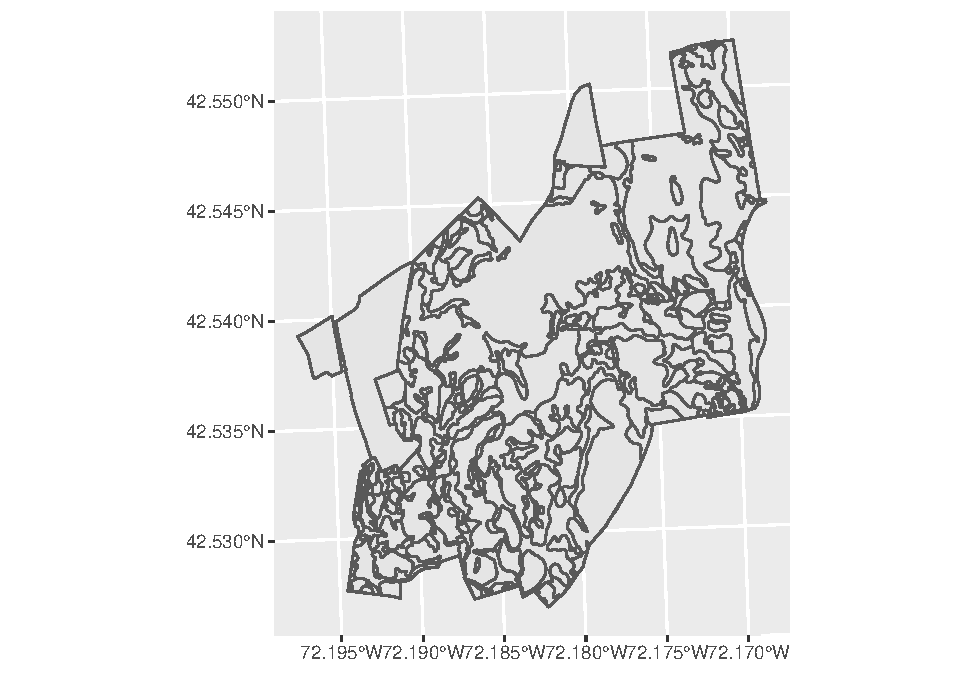
\includegraphics{ConservationGIS_files/figure-latex/unnamed-chunk-6-1.pdf}

GIS maps are all about ``layers'' of data. The order in which data are displayed in \texttt{ggplot} is important. In the above code, we ``layered'' the \texttt{HARV\_soils} polygon \emph{over} the \texttt{HARV\_boundary} polygon. Check what happens when we layer them in the opposite order:

\begin{Shaded}
\begin{Highlighting}[]
\FunctionTok{ggplot}\NormalTok{() }\SpecialCharTok{+}
  \FunctionTok{geom\_sf}\NormalTok{(}\AttributeTok{data =}\NormalTok{ HARV\_soils) }\SpecialCharTok{+} 
  \FunctionTok{geom\_sf}\NormalTok{(}\AttributeTok{data =}\NormalTok{ HARV\_boundary)}
\end{Highlighting}
\end{Shaded}

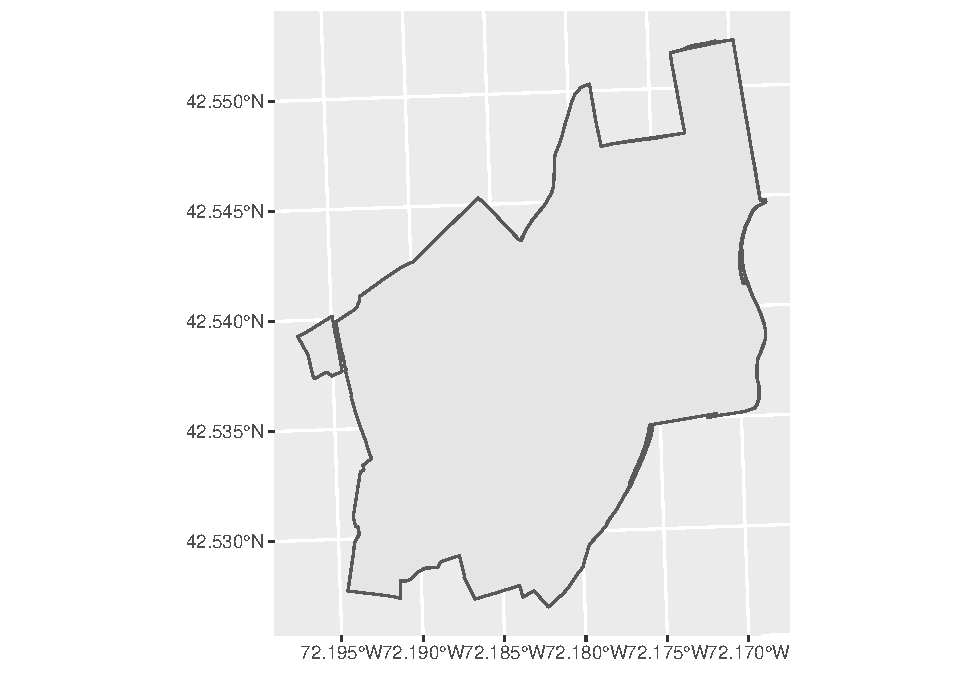
\includegraphics{ConservationGIS_files/figure-latex/unnamed-chunk-7-1.pdf}

Now the boundary file is over top the soils one and because it is a filled polygon, we can't see the soils layer. One way we can deal with this, is by adjusting the transparency of the boundary layer with the \texttt{alpha} function. This adjusts the transparency from fully transparent (\texttt{alpha\ =\ 0}), to fully opaque (\texttt{alpha\ =\ 1}).

\begin{Shaded}
\begin{Highlighting}[]
\FunctionTok{ggplot}\NormalTok{() }\SpecialCharTok{+}
  \FunctionTok{geom\_sf}\NormalTok{(}\AttributeTok{data =}\NormalTok{ HARV\_soils) }\SpecialCharTok{+} 
  \FunctionTok{geom\_sf}\NormalTok{(}\AttributeTok{data =}\NormalTok{ HARV\_boundary, }\AttributeTok{alpha =} \FloatTok{0.1}\NormalTok{)}
\end{Highlighting}
\end{Shaded}

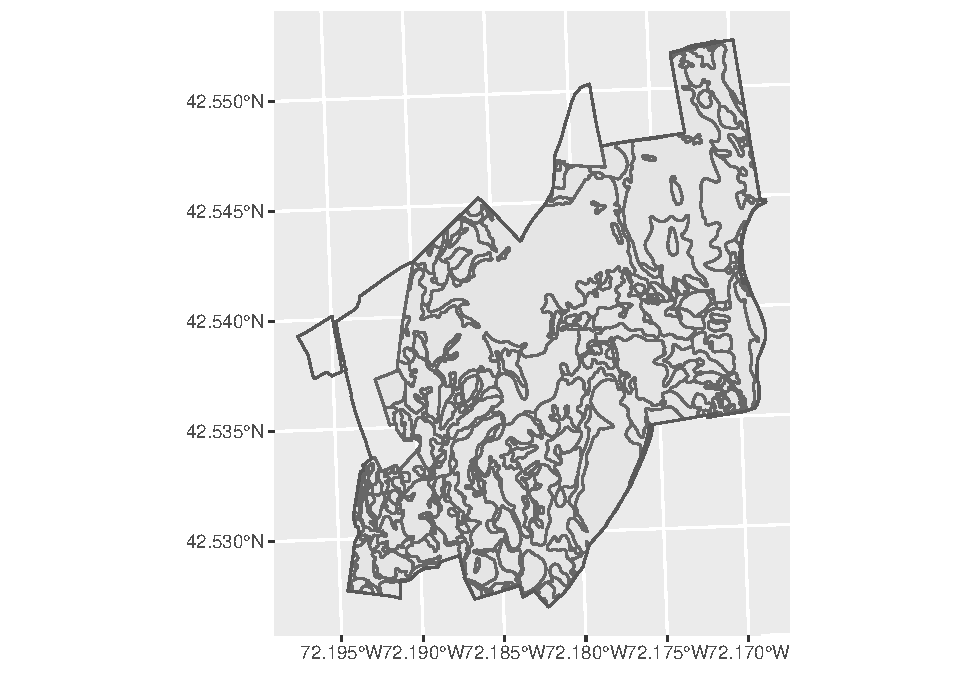
\includegraphics{ConservationGIS_files/figure-latex/unnamed-chunk-8-1.pdf}

We can also symbolize data based on the attributes. Before we do that, let's explore the HARV\_soils layer. If you type \texttt{HARV\_soils} At the \texttt{\textgreater{}} prompt, you will see the metadata. You will see that in addition to some descriptions of the geographic reference system (for more on that, see the chapter \ref{projections}), you will see some attributes, including different kinds of soil classification and drainage types. If we want to display the soil polygons by their SIMMONS\_SO field, we would use the \texttt{aes} (for aesthetics) function.

\begin{Shaded}
\begin{Highlighting}[]
\FunctionTok{ggplot}\NormalTok{() }\SpecialCharTok{+}
  \FunctionTok{geom\_sf}\NormalTok{(}\AttributeTok{data =}\NormalTok{ HARV\_soils, }\AttributeTok{mapping =} \FunctionTok{aes}\NormalTok{(}\AttributeTok{fill =}\NormalTok{ SIMMONS\_SO)) }\SpecialCharTok{+} 
  \FunctionTok{geom\_sf}\NormalTok{(}\AttributeTok{data =}\NormalTok{ HARV\_boundary, }\AttributeTok{alpha =} \FloatTok{0.1}\NormalTok{)}
\end{Highlighting}
\end{Shaded}

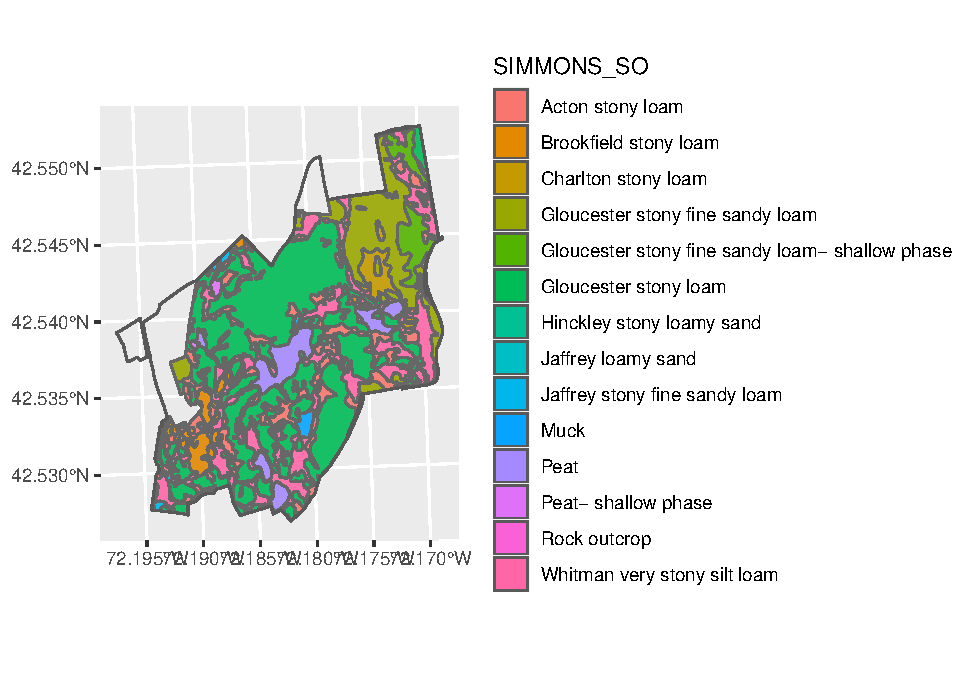
\includegraphics{ConservationGIS_files/figure-latex/unnamed-chunk-9-1.pdf}

The default colour scheme has been applied. You can change this using different built in colour maps. Below is the code to use the \texttt{viridis} colour map.

\begin{Shaded}
\begin{Highlighting}[]
\FunctionTok{ggplot}\NormalTok{() }\SpecialCharTok{+}
  \FunctionTok{geom\_sf}\NormalTok{(}\AttributeTok{data =}\NormalTok{ HARV\_soils, }\AttributeTok{mapping =} \FunctionTok{aes}\NormalTok{(}\AttributeTok{fill =}\NormalTok{ SIMMONS\_SO)) }\SpecialCharTok{+} 
  \FunctionTok{geom\_sf}\NormalTok{(}\AttributeTok{data =}\NormalTok{ HARV\_boundary, }\AttributeTok{alpha =} \FloatTok{0.1}\NormalTok{) }\SpecialCharTok{+}
  \FunctionTok{scale\_fill\_viridis\_d}\NormalTok{()}
\end{Highlighting}
\end{Shaded}

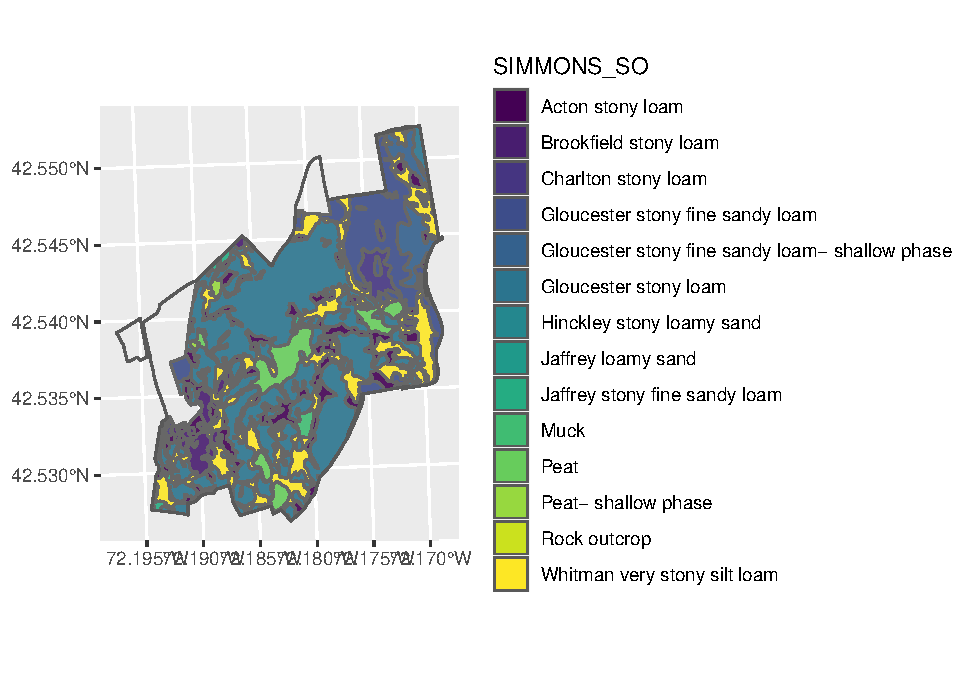
\includegraphics{ConservationGIS_files/figure-latex/unnamed-chunk-10-1.pdf}

To see other aesthetics that can be modified, run \texttt{vignette("ggplot2-specs")}

\hypertarget{raster}{%
\chapter{Reading in Raster Data}\label{raster}}

We will use the R package \texttt{stars} for handling raster data. You will have to download and install this package from the CRAN repository (review section \href{https://ahurford.github.io/quant-guide-all-courses/rintro.html\#r-packages}{4.10} of the MUN Biology R manual if need a reminder of how to do this).

\begin{Shaded}
\begin{Highlighting}[]
\FunctionTok{library}\NormalTok{(stars) }
\end{Highlighting}
\end{Shaded}

To plot the data (i.e., make a map) we will also need the package \texttt{ggplot2}, so make sure to load and install that as well, if you haven't yet already.

\begin{Shaded}
\begin{Highlighting}[]
\FunctionTok{library}\NormalTok{(ggplot2)}
\end{Highlighting}
\end{Shaded}

If you didn't already set the working directory to where you have downloaded the HARV folder, do so now. This folder contains 4 .tif files. You may be familiar with .tif files as digital photographs. These are a special kind of .tif called a geotiff. Like a digital photograph, it has pixels, but it also has georeferenced data.

We will read in the raster that represents the digital terrain model (dtm for short) - in this raster, each pixel gives the elevation above sea level of that point. We use the \texttt{read\_stars} function.

\begin{Shaded}
\begin{Highlighting}[]
\NormalTok{HARV\_dtm }\OtherTok{\textless{}{-}} \FunctionTok{read\_stars}\NormalTok{(}\StringTok{"HARV/HARV\_dtmFull.tif"}\NormalTok{)}
\end{Highlighting}
\end{Shaded}

To plot it, we use \texttt{geom\_stars()} in \texttt{ggplot()}. We'll use the \texttt{viridis} colour palette. Note that we specified \_c (for continous) here, because the raster values are continuous data, whereas when we used the colour palette for the soils polygon data in the \ref{vector} chapter, we used \_d (for discrete), because those data were discrete categories.

\begin{Shaded}
\begin{Highlighting}[]
\FunctionTok{ggplot}\NormalTok{() }\SpecialCharTok{+}
  \FunctionTok{geom\_stars}\NormalTok{(}\AttributeTok{data =}\NormalTok{ HARV\_dtm) }\SpecialCharTok{+}
  \FunctionTok{scale\_fill\_viridis\_c}\NormalTok{()}
\end{Highlighting}
\end{Shaded}

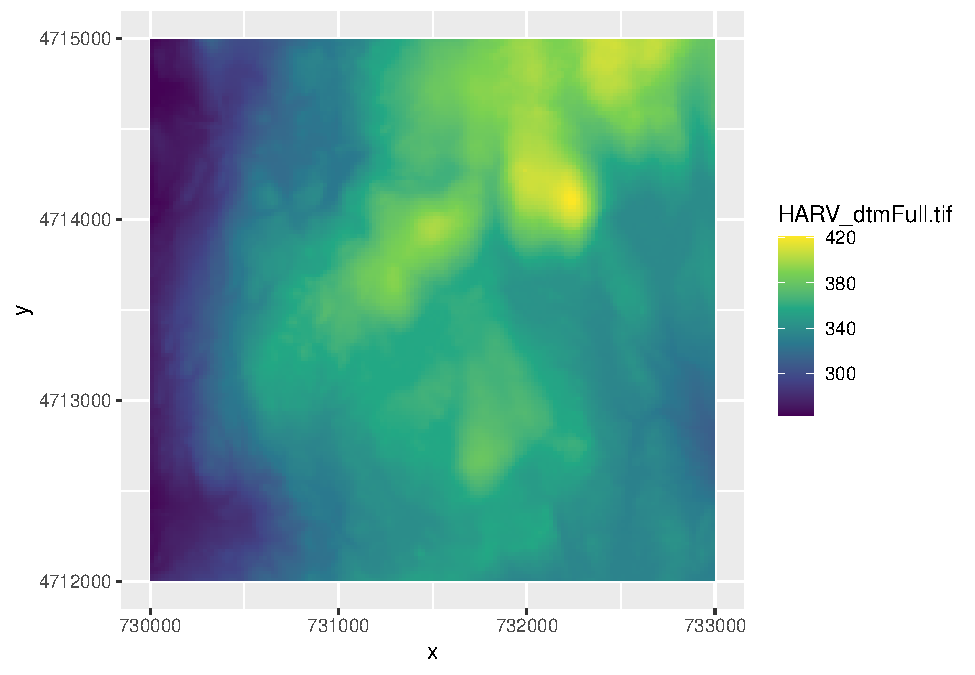
\includegraphics{ConservationGIS_files/figure-latex/unnamed-chunk-15-1.pdf}

\textbf{NOTE}: If it takes too long to draw the map, try loading in a subset of the dtm (the ``HARV\_DTMCrop.tif'' file) instead. Raster files can take a long time to load and depending on your computer's available CPU, you may wish to use a smaller raster layer)

What if we want to show the boundaries of the Harvard forest on top of this raster layer? Add it in ggplot like this:

\begin{Shaded}
\begin{Highlighting}[]
\FunctionTok{ggplot}\NormalTok{() }\SpecialCharTok{+}
  \FunctionTok{geom\_stars}\NormalTok{(}\AttributeTok{data =}\NormalTok{ HARV\_dtm) }\SpecialCharTok{+}
  \FunctionTok{geom\_sf}\NormalTok{(}\AttributeTok{data =}\NormalTok{ HARV\_boundary, }\AttributeTok{alpha =} \FloatTok{0.1}\NormalTok{) }\SpecialCharTok{+}
  \FunctionTok{scale\_fill\_viridis\_c}\NormalTok{()}
\end{Highlighting}
\end{Shaded}

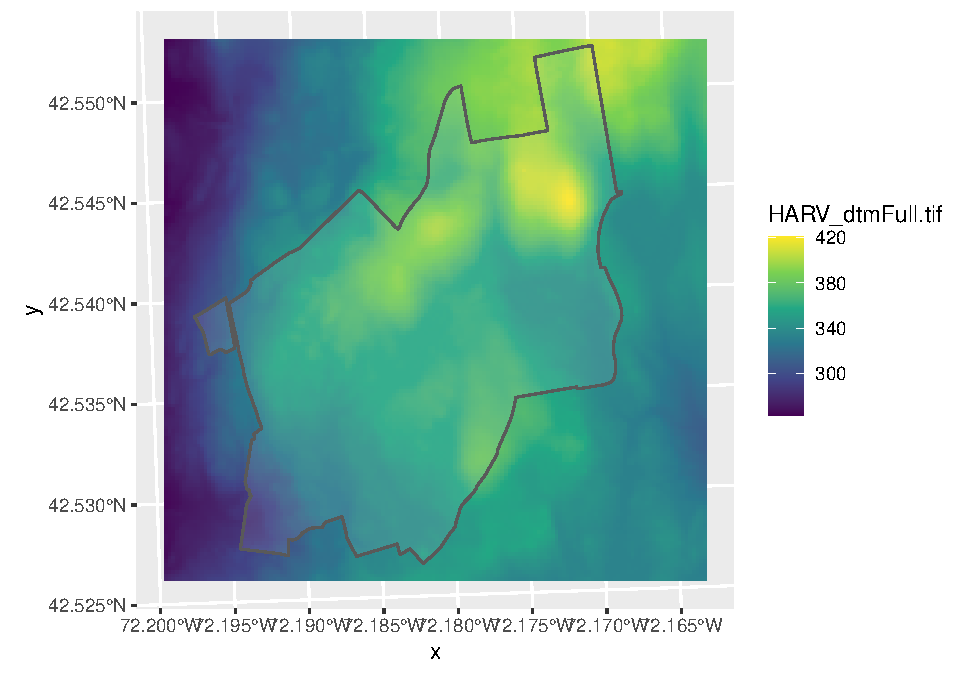
\includegraphics{ConservationGIS_files/figure-latex/unnamed-chunk-16-1.pdf}

Let's try making another map that combines raster and vector data. Download the SJER folder, and change your working directory to that folder. This is similar data to that from the Harvard forest, but from the San Joaquin Experimental Range. On your own, read in the following layers and try to plot them.
1. sjer\_plots (these are point files that represent the location of the sample plots)
1. SJER\_dtmFULL.tif (a raster of the digital terrain model showing elevations)

\begin{Shaded}
\begin{Highlighting}[]
\NormalTok{SJER\_plots }\OtherTok{\textless{}{-}} \FunctionTok{st\_read}\NormalTok{(}\StringTok{"SJER/sjer\_plots.shp"}\NormalTok{)}
\end{Highlighting}
\end{Shaded}

\begin{verbatim}
## Reading layer `sjer_plots' from data source `C:\Users\ywiersma\Documents\BIOL4651\GIS_R_manual\ConsBiol_SpatialAnalysis\SJER\sjer_plots.shp' using driver `ESRI Shapefile'
## Simple feature collection with 7 features and 2 fields
## geometry type:  POINT
## dimension:      XY
## bbox:           xmin: -119.7432 ymin: 37.10542 xmax: -119.7298 ymax: 37.11729
## geographic CRS: WGS 84
\end{verbatim}

\begin{Shaded}
\begin{Highlighting}[]
\NormalTok{SJER\_dtm }\OtherTok{\textless{}{-}} \FunctionTok{read\_stars}\NormalTok{(}\StringTok{"SJER/SJER\_dtmFULL.tif"}\NormalTok{)}

\FunctionTok{ggplot}\NormalTok{() }\SpecialCharTok{+}
  \FunctionTok{geom\_stars}\NormalTok{(}\AttributeTok{data =}\NormalTok{ SJER\_dtm) }\SpecialCharTok{+}
  \FunctionTok{geom\_sf}\NormalTok{(}\AttributeTok{data =}\NormalTok{ SJER\_plots)}
\end{Highlighting}
\end{Shaded}

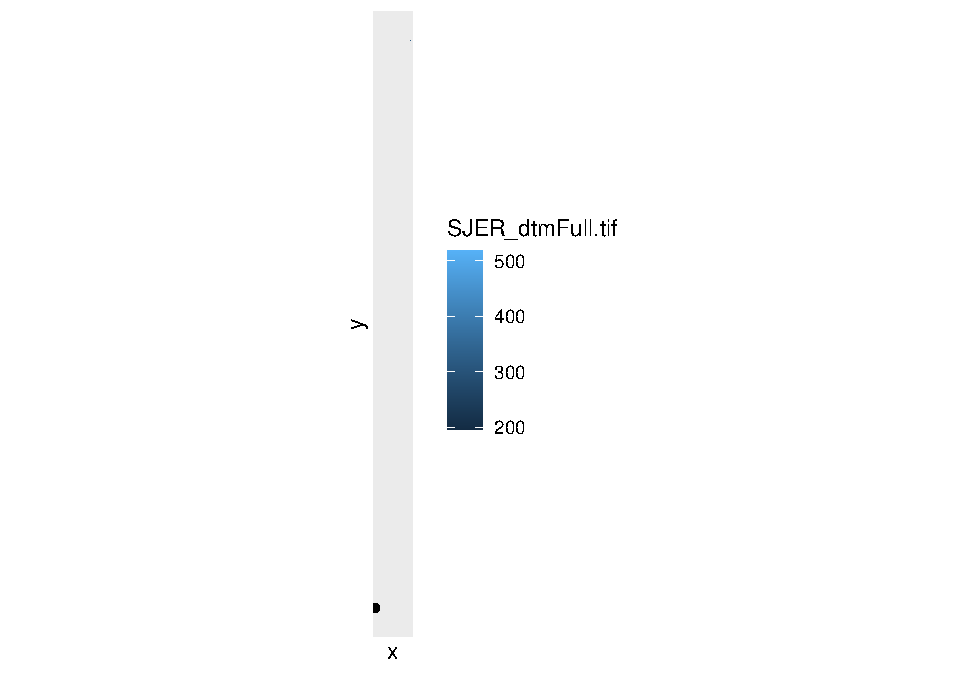
\includegraphics{ConservationGIS_files/figure-latex/unnamed-chunk-18-1.pdf}

You will get a map that does not quite look right. Congratulations - you've discovered the most common (and frustrating) issue with spatial data - conflicting projections. To learn more, go the the chapter on projections; chapter \ref{projections}.

\hypertarget{projections}{%
\chapter{Dealing with Projections}\label{projections}}

At the end of the vectors \ref{vector} chapter, we tried to map the plots layer for the San Joaquin Experimental Range over the digital terrain model (dtm). The two layers didn't display properly, so something went wrong. To see what happened, we need to have a look at the co-ordinate reference system (crs) for the two layers. Use the \texttt{st\_crs} command to see what this is for each layer.

\begin{Shaded}
\begin{Highlighting}[]
\FunctionTok{st\_crs}\NormalTok{(SJER\_plots)}
\end{Highlighting}
\end{Shaded}

\begin{verbatim}
## Coordinate Reference System:
##   User input: WGS 84 
##   wkt:
## GEOGCRS["WGS 84",
##     DATUM["World Geodetic System 1984",
##         ELLIPSOID["WGS 84",6378137,298.257223563,
##             LENGTHUNIT["metre",1]]],
##     PRIMEM["Greenwich",0,
##         ANGLEUNIT["degree",0.0174532925199433]],
##     CS[ellipsoidal,2],
##         AXIS["latitude",north,
##             ORDER[1],
##             ANGLEUNIT["degree",0.0174532925199433]],
##         AXIS["longitude",east,
##             ORDER[2],
##             ANGLEUNIT["degree",0.0174532925199433]],
##     ID["EPSG",4326]]
\end{verbatim}

\begin{Shaded}
\begin{Highlighting}[]
\FunctionTok{st\_crs}\NormalTok{(SJER\_dtm)}
\end{Highlighting}
\end{Shaded}

\begin{verbatim}
## Coordinate Reference System:
##   User input: WGS 84 / UTM zone 11N 
##   wkt:
## PROJCRS["WGS 84 / UTM zone 11N",
##     BASEGEOGCRS["WGS 84",
##         DATUM["World Geodetic System 1984",
##             ELLIPSOID["WGS 84",6378137,298.257223563,
##                 LENGTHUNIT["metre",1]]],
##         PRIMEM["Greenwich",0,
##             ANGLEUNIT["degree",0.0174532925199433]],
##         ID["EPSG",4326]],
##     CONVERSION["UTM zone 11N",
##         METHOD["Transverse Mercator",
##             ID["EPSG",9807]],
##         PARAMETER["Latitude of natural origin",0,
##             ANGLEUNIT["degree",0.0174532925199433],
##             ID["EPSG",8801]],
##         PARAMETER["Longitude of natural origin",-117,
##             ANGLEUNIT["degree",0.0174532925199433],
##             ID["EPSG",8802]],
##         PARAMETER["Scale factor at natural origin",0.9996,
##             SCALEUNIT["unity",1],
##             ID["EPSG",8805]],
##         PARAMETER["False easting",500000,
##             LENGTHUNIT["metre",1],
##             ID["EPSG",8806]],
##         PARAMETER["False northing",0,
##             LENGTHUNIT["metre",1],
##             ID["EPSG",8807]]],
##     CS[Cartesian,2],
##         AXIS["(E)",east,
##             ORDER[1],
##             LENGTHUNIT["metre",1]],
##         AXIS["(N)",north,
##             ORDER[2],
##             LENGTHUNIT["metre",1]],
##     USAGE[
##         SCOPE["unknown"],
##         AREA["World - N hemisphere - 120°W to 114°W - by country"],
##         BBOX[0,-120,84,-114]],
##     ID["EPSG",32611]]
\end{verbatim}

Scroll through the results and compare the last set of numbers at the end of the file in the ID{[}{]} line. You should note that the SJER\_plots file as an ID of 4325 and that the SJER\_dtm has an ID of 32611. This indicates that the two layers have different coordinate systems. You can verify this by plotting each separately and cheeking the coordinate system labels on the map edges. The labels on the dtm are in UTM units, while the labels on the plots are in latitude and longitude. We need to convert the coordinate reference system (crs) of one of the layers to match the other. We use the \texttt{st\_transform} function to create a new plots layer which has a projection system that matches the dtm layer.

\begin{Shaded}
\begin{Highlighting}[]
\NormalTok{SJER\_plots\_utm }\OtherTok{\textless{}{-}} \FunctionTok{st\_transform}\NormalTok{(SJER\_plots, }\FunctionTok{st\_crs}\NormalTok{(SJER\_dtm))}
\end{Highlighting}
\end{Shaded}

Now you should be able to plot the two layers together

\begin{Shaded}
\begin{Highlighting}[]
\FunctionTok{ggplot}\NormalTok{() }\SpecialCharTok{+}
  \FunctionTok{geom\_stars}\NormalTok{(}\AttributeTok{data =}\NormalTok{ SJER\_dtm) }\SpecialCharTok{+}
  \FunctionTok{geom\_sf}\NormalTok{(}\AttributeTok{data =}\NormalTok{ SJER\_plots\_utm)}
\end{Highlighting}
\end{Shaded}

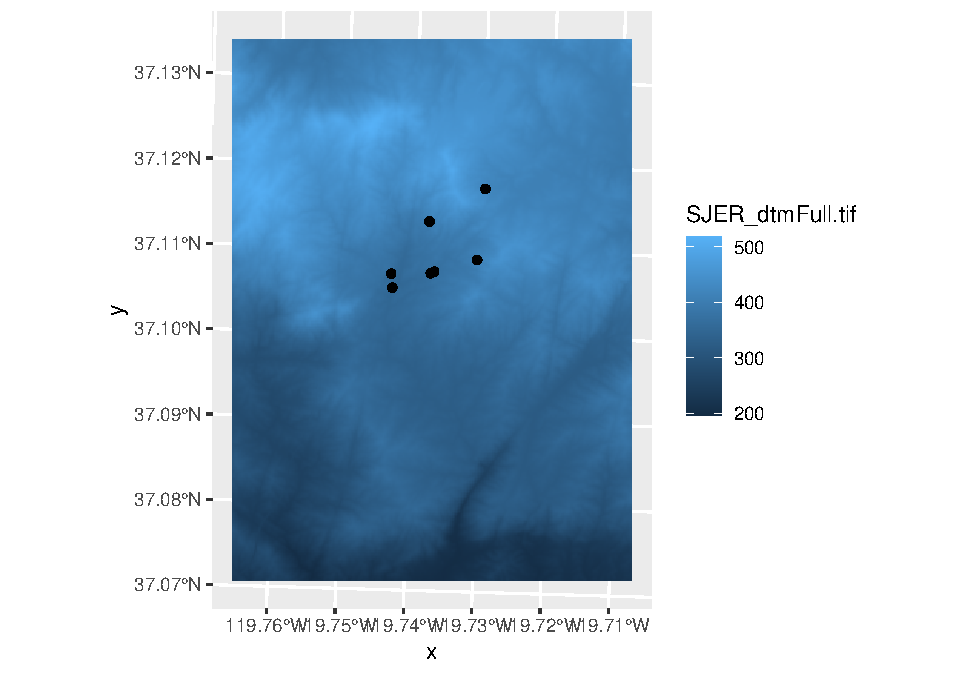
\includegraphics{ConservationGIS_files/figure-latex/unnamed-chunk-21-1.pdf}

Now that you have the two data sets aligned, you can extract the elevation data for each point, which is explained in the chapter on extracting data \ref{extractingData}. Before you do that, complete the exercises in the next chapter \ref{rasterAlgebra}.

\hypertarget{rasterAlgebra}{%
\chapter{Raster Algebra}\label{rasterAlgebra}}

It is possible to analyse and combine two different rasters. The second raster layer in the SJER folder is a digital surface model (dsm) which is a data set taken using Lidar data that measures the height of the objects (above sea level) of objects on the earth. Let's load that layer.

\begin{Shaded}
\begin{Highlighting}[]
\NormalTok{SJER\_dsm }\OtherTok{\textless{}{-}} \FunctionTok{read\_stars}\NormalTok{(}\StringTok{"SJER/SJER\_dsmCROP.tif"}\NormalTok{)}
\end{Highlighting}
\end{Shaded}

By subtracting the dtm (elevation of the ground above sea level) from the dsm (elevation of the objects on the ground above sea level) we can create a new raster that represents the height of those objects above the ground. Since this layer is in a forest, we can infer that this new layer is the canopy height. However, the dsm layer covers a smaller extent that the dtm, so we'll also read in the cropped .tif file for the dtm

\begin{Shaded}
\begin{Highlighting}[]
\NormalTok{SJER\_dtm\_cropped }\OtherTok{\textless{}{-}} \FunctionTok{read\_stars}\NormalTok{(}\StringTok{"SJER/SJER\_dtmCROP.tif"}\NormalTok{)}
\end{Highlighting}
\end{Shaded}

Now we can do the raster algebra:

\begin{Shaded}
\begin{Highlighting}[]
\NormalTok{SJER\_canopy }\OtherTok{=}\NormalTok{ SJER\_dsm }\SpecialCharTok{{-}}\NormalTok{ SJER\_dtm\_cropped}
\end{Highlighting}
\end{Shaded}

Raster algebra can use any algebraic functions and involve one or more raster layers - for example if we wanted to convert the units of the canopy layer from metres to centimetres, we could simply multiply the SJER\_canopy layer by 10. Or if you had a raster of canopy height in 2000 and canopy height in 2020, you could subtract one from the other to find out how much the tree height changed over 20 years in different parts of the landscape.

Now we can extract the canopy height data from our sample locations - see chapter \ref{extractingData}.

\hypertarget{extractingData}{%
\chapter{Extracting Data from a Raster}\label{extractingData}}

A common thing that ecologists and conservation biologists want to get data for their sample sites from different GIS layers and then use these data in different models or statistical tests.

\hypertarget{sampling-data-from-a-raster-using-points}{%
\section{Sampling data from a raster using points}\label{sampling-data-from-a-raster-using-points}}

We use the \texttt{aggregate} function to get data from the canopy raster

\begin{Shaded}
\begin{Highlighting}[]
\NormalTok{plot\_canopy\_height }\OtherTok{\textless{}{-}} \FunctionTok{aggregate}\NormalTok{(SJER\_canopy, SJER\_plots\_utm, mean, }\AttributeTok{as\_points =} \ConstantTok{FALSE}\NormalTok{)}
\NormalTok{plot\_canopy\_height}\SpecialCharTok{$}\NormalTok{SJER\_dsmCrop.tif}
\end{Highlighting}
\end{Shaded}

\begin{verbatim}
## [1] 18.913757 23.948151  1.986877  2.183136 28.985016  3.506866  2.201233
\end{verbatim}

To link this data into the attribute data we will use the \texttt{mutate} function in the package \texttt{dplyr}. We have a lab in BIOL 1002 that teaches some of the basics of the dplyr package. If you're not familiar with that package, just use the code below.

\begin{Shaded}
\begin{Highlighting}[]
\FunctionTok{library}\NormalTok{(dplyr)}
\end{Highlighting}
\end{Shaded}

\begin{Shaded}
\begin{Highlighting}[]
\FunctionTok{mutate}\NormalTok{(SJER\_plots\_utm, }\AttributeTok{canopyHeight =}\NormalTok{ plot\_canopy\_height}\SpecialCharTok{$}\NormalTok{SJER\_dsmCrop.tif)}
\end{Highlighting}
\end{Shaded}

\begin{verbatim}
## Simple feature collection with 7 features and 3 fields
## geometry type:  POINT
## dimension:      XY
## bbox:           xmin: 256238.5 ymin: 4110088 xmax: 257465.5 ymax: 4111372
## projected CRS:  WGS 84 / UTM zone 11N
##   plot_id   plot_type                 geometry canopyHeight
## 1       1       Tower POINT (257465.5 4111372)    18.913757
## 2       2       Tower POINT (256238.5 4110270)    23.948151
## 3       3       Tower POINT (256798.3 4110296)     1.986877
## 4       4 Distributed POINT (256737.7 4110949)     2.183136
## 5       5 Distributed POINT (257358.5 4110450)    28.985016
## 6       6 Distributed POINT (256254.5 4110088)     3.506866
## 7       7 Distributed POINT (256754.5 4110274)     2.201233
\end{verbatim}

If you examine the SJER\_plots\_utm data, you will see that it now has the canopy height data in the attribute data. You'll notice that there is also an attribute for \texttt{plot\_type}. We can make a map that symbolizes the sample points by the plot type like this:

\begin{Shaded}
\begin{Highlighting}[]
\FunctionTok{ggplot}\NormalTok{() }\SpecialCharTok{+}
  \FunctionTok{geom\_stars}\NormalTok{(}\AttributeTok{data =}\NormalTok{ SJER\_canopy) }\SpecialCharTok{+}
  \FunctionTok{geom\_sf}\NormalTok{(}\AttributeTok{data =}\NormalTok{ SJER\_plots\_utm, }\AttributeTok{mapping =} \FunctionTok{aes}\NormalTok{(}\AttributeTok{color =}\NormalTok{ plot\_type))}
\end{Highlighting}
\end{Shaded}

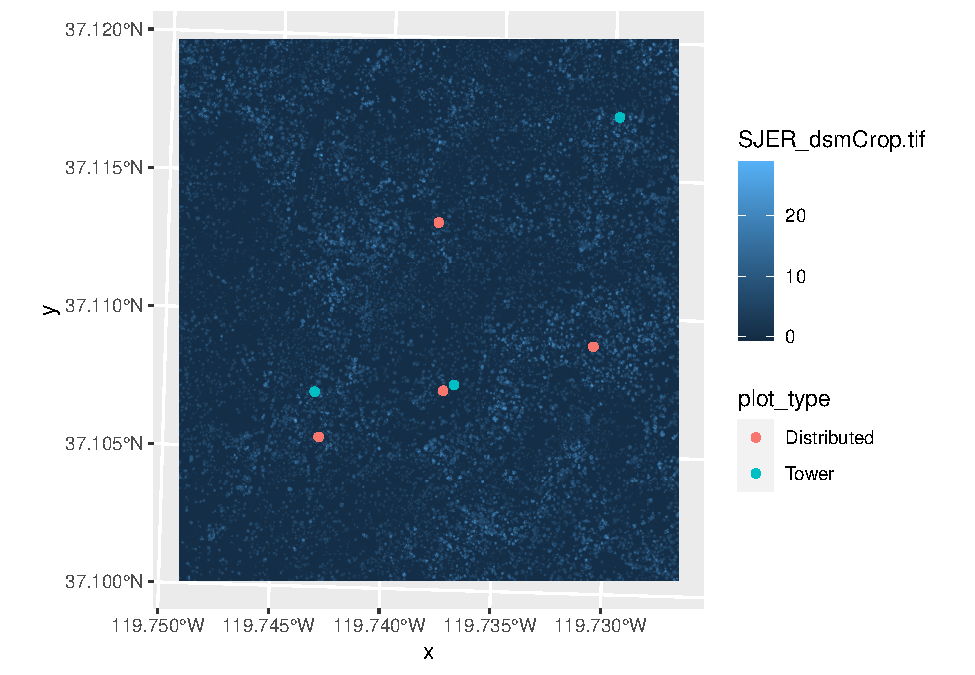
\includegraphics{ConservationGIS_files/figure-latex/unnamed-chunk-28-1.pdf}

You could now take this data and test whether canopy height is significantly different at the tower sampling points or at the distributed sampling points. We won't do that just now; we'll do some statistics on these data in a different module.

\hypertarget{sampling-data-from-a-raster-using-polygons}{%
\section{Sampling data from a raster using polygons}\label{sampling-data-from-a-raster-using-polygons}}

At other times, researchers may want to sample data from a raster using a polygon. For example, we might want to know what the maximum elevation within the boundaries of a protected area is.

To do these exercises, we're going to change back to Harvard forest data set. Set your working directory to the HARV folder.

We're going to find out what the maximum elevation is in each of the soil drainage polygons.

First, check that the two layers have the same co-ordinate reference system:

\begin{Shaded}
\begin{Highlighting}[]
\FunctionTok{st\_crs}\NormalTok{(HARV\_dtm)}
\end{Highlighting}
\end{Shaded}

\begin{verbatim}
## Coordinate Reference System:
##   User input: WGS 84 / UTM zone 18N 
##   wkt:
## PROJCRS["WGS 84 / UTM zone 18N",
##     BASEGEOGCRS["WGS 84",
##         DATUM["World Geodetic System 1984",
##             ELLIPSOID["WGS 84",6378137,298.257223563,
##                 LENGTHUNIT["metre",1]]],
##         PRIMEM["Greenwich",0,
##             ANGLEUNIT["degree",0.0174532925199433]],
##         ID["EPSG",4326]],
##     CONVERSION["UTM zone 18N",
##         METHOD["Transverse Mercator",
##             ID["EPSG",9807]],
##         PARAMETER["Latitude of natural origin",0,
##             ANGLEUNIT["degree",0.0174532925199433],
##             ID["EPSG",8801]],
##         PARAMETER["Longitude of natural origin",-75,
##             ANGLEUNIT["degree",0.0174532925199433],
##             ID["EPSG",8802]],
##         PARAMETER["Scale factor at natural origin",0.9996,
##             SCALEUNIT["unity",1],
##             ID["EPSG",8805]],
##         PARAMETER["False easting",500000,
##             LENGTHUNIT["metre",1],
##             ID["EPSG",8806]],
##         PARAMETER["False northing",0,
##             LENGTHUNIT["metre",1],
##             ID["EPSG",8807]]],
##     CS[Cartesian,2],
##         AXIS["(E)",east,
##             ORDER[1],
##             LENGTHUNIT["metre",1]],
##         AXIS["(N)",north,
##             ORDER[2],
##             LENGTHUNIT["metre",1]],
##     USAGE[
##         SCOPE["unknown"],
##         AREA["World - N hemisphere - 78°W to 72°W - by country"],
##         BBOX[0,-78,84,-72]],
##     ID["EPSG",32618]]
\end{verbatim}

\begin{Shaded}
\begin{Highlighting}[]
\FunctionTok{st\_crs}\NormalTok{(HARV\_soils)}
\end{Highlighting}
\end{Shaded}

\begin{verbatim}
## Coordinate Reference System:
##   User input: WGS 84 / UTM zone 18N 
##   wkt:
## PROJCRS["WGS 84 / UTM zone 18N",
##     BASEGEOGCRS["WGS 84",
##         DATUM["World Geodetic System 1984",
##             ELLIPSOID["WGS 84",6378137,298.257223563,
##                 LENGTHUNIT["metre",1]]],
##         PRIMEM["Greenwich",0,
##             ANGLEUNIT["degree",0.0174532925199433]],
##         ID["EPSG",4326]],
##     CONVERSION["UTM zone 18N",
##         METHOD["Transverse Mercator",
##             ID["EPSG",9807]],
##         PARAMETER["Latitude of natural origin",0,
##             ANGLEUNIT["Degree",0.0174532925199433],
##             ID["EPSG",8801]],
##         PARAMETER["Longitude of natural origin",-75,
##             ANGLEUNIT["Degree",0.0174532925199433],
##             ID["EPSG",8802]],
##         PARAMETER["Scale factor at natural origin",0.9996,
##             SCALEUNIT["unity",1],
##             ID["EPSG",8805]],
##         PARAMETER["False easting",500000,
##             LENGTHUNIT["metre",1],
##             ID["EPSG",8806]],
##         PARAMETER["False northing",0,
##             LENGTHUNIT["metre",1],
##             ID["EPSG",8807]]],
##     CS[Cartesian,2],
##         AXIS["(E)",east,
##             ORDER[1],
##             LENGTHUNIT["metre",1]],
##         AXIS["(N)",north,
##             ORDER[2],
##             LENGTHUNIT["metre",1]],
##     ID["EPSG",32618]]
\end{verbatim}

The ID code at the end of each file is identical (\texttt{32618}), so you can overlay these layers and extract the data. If you are not convinced, try mapping them together.

Then we use the same \texttt{aggregate} function as we did to extract the data from the raster to points. Note, that when you extract with a polygon, there are many pixels within the polygon. You can specify different values you want to extract from the pixels within the polygon, for example, maximum, minimum, mean.

\begin{Shaded}
\begin{Highlighting}[]
\NormalTok{drainage\_max\_elev }\OtherTok{\textless{}{-}} \FunctionTok{aggregate}\NormalTok{(HARV\_dtm, HARV\_soils, max, }\AttributeTok{as\_points =} \ConstantTok{FALSE}\NormalTok{)}
\NormalTok{drainage\_max\_elev}\SpecialCharTok{$}\NormalTok{HARv\_dtmFull.tif}
\end{Highlighting}
\end{Shaded}

\begin{verbatim}
## NULL
\end{verbatim}

Here we'll use the \texttt{mutate} function and create a new shapefile

\begin{Shaded}
\begin{Highlighting}[]
\NormalTok{elevation\_by\_drainage }\OtherTok{\textless{}{-}} \FunctionTok{mutate}\NormalTok{(HARV\_soils, }\AttributeTok{elevation =}\NormalTok{ drainage\_max\_elev}\SpecialCharTok{$}\NormalTok{HARV\_dtmFull.tif)}
\end{Highlighting}
\end{Shaded}

Now we can plot the soil drainage basins and colour code them by their maximum height.

\begin{Shaded}
\begin{Highlighting}[]
\FunctionTok{ggplot}\NormalTok{() }\SpecialCharTok{+}
  \FunctionTok{geom\_sf}\NormalTok{(}\AttributeTok{data =}\NormalTok{ elevation\_by\_drainage, }\AttributeTok{mapping =} \FunctionTok{aes}\NormalTok{(}\AttributeTok{fill =}\NormalTok{ elevation)) }\SpecialCharTok{+}
  \FunctionTok{scale\_fill\_viridis\_c}\NormalTok{()}
\end{Highlighting}
\end{Shaded}

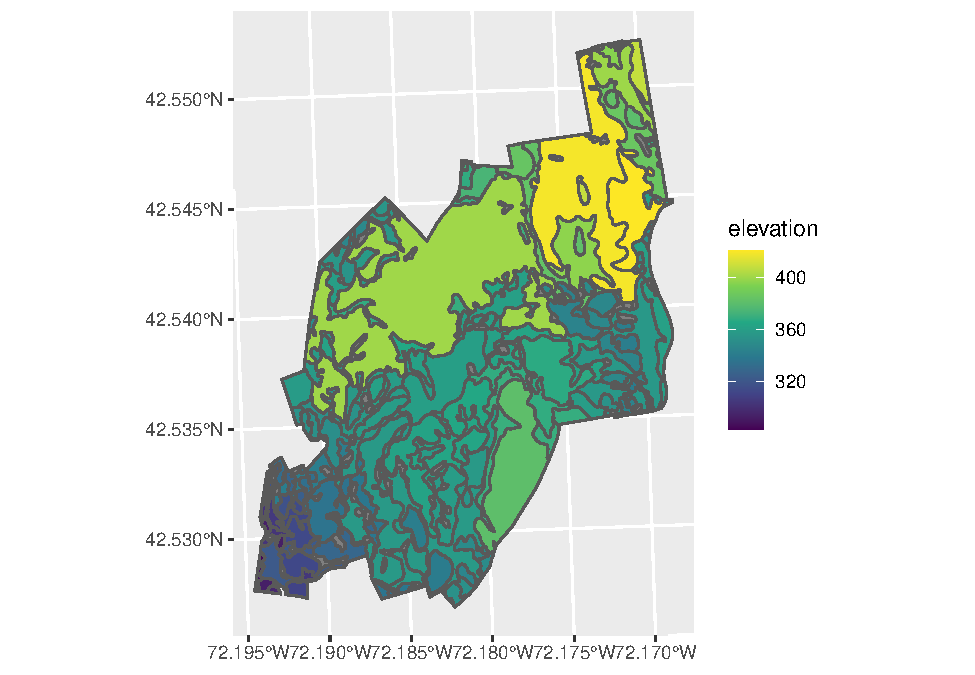
\includegraphics{ConservationGIS_files/figure-latex/unnamed-chunk-33-1.pdf}

If you want to change the map display so the coordinates on the map boundary are in UTM, you can do it like so:

\begin{Shaded}
\begin{Highlighting}[]
\FunctionTok{ggplot}\NormalTok{() }\SpecialCharTok{+}
  \FunctionTok{geom\_sf}\NormalTok{(}\AttributeTok{data =}\NormalTok{ elevation\_by\_drainage, }\AttributeTok{mapping =} \FunctionTok{aes}\NormalTok{(}\AttributeTok{fill =}\NormalTok{ elevation)) }\SpecialCharTok{+}
  \FunctionTok{coord\_sf}\NormalTok{(}\AttributeTok{datum =} \FunctionTok{st\_crs}\NormalTok{(HARV\_dtm)) }\SpecialCharTok{+} 
  \FunctionTok{scale\_fill\_viridis\_c}\NormalTok{()}
\end{Highlighting}
\end{Shaded}

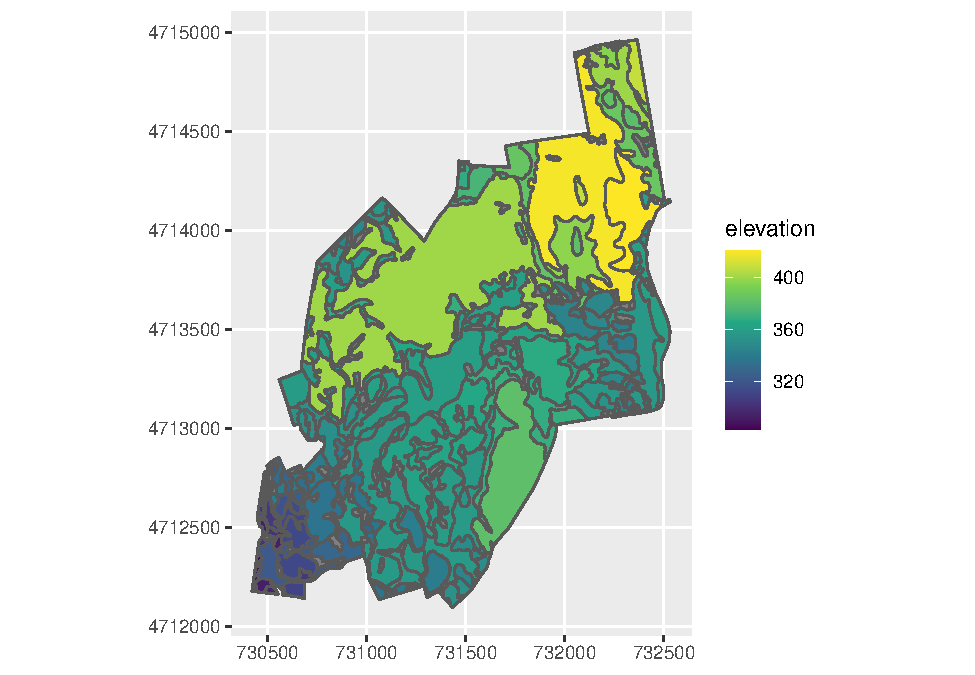
\includegraphics{ConservationGIS_files/figure-latex/unnamed-chunk-34-1.pdf}

What if you have sampled points in the field with a handheld gps and only have a csv file with x and y coordinates? How can you get the data? Go to chapter \ref{PointsData} to find out!

\hypertarget{PointsData}{%
\chapter{Creating a Points Shapefile from Data}\label{PointsData}}

Often you will have a .csv file with x and y coordinates (either in lat/lon or UTM) that you sampled in the field and want to load into a GIS so that you can extract data from other GIS layers. Here's how to do it. We'll jump back to the San Joaquin Data set, so reset your working directory to the SJER folder (you're getting lots of practice with working directories this way!)

First we need to load the csv plots data as an `\texttt{sf} object and display it

\begin{Shaded}
\begin{Highlighting}[]
\NormalTok{plots\_sjer\_csv }\OtherTok{\textless{}{-}} \FunctionTok{st\_read}\NormalTok{(}\StringTok{"SJER/sjer\_plots.csv"}\NormalTok{, }\AttributeTok{options =} \FunctionTok{c}\NormalTok{(}\StringTok{"X\_POSSIBLE\_NAMES=longitude"}\NormalTok{, }\StringTok{"Y\_POSSIBLE\_NAMES=latitude"}\NormalTok{), }\AttributeTok{crs =} \DecValTok{4326}\NormalTok{)}
\end{Highlighting}
\end{Shaded}

\begin{verbatim}
## options:        X_POSSIBLE_NAMES=longitude Y_POSSIBLE_NAMES=latitude 
## Reading layer `sjer_plots' from data source `C:\Users\ywiersma\Documents\BIOL4651\GIS_R_manual\ConsBiol_SpatialAnalysis\SJER\sjer_plots.csv' using driver `CSV'
## Simple feature collection with 7 features and 4 fields
## geometry type:  POINT
## dimension:      XY
## bbox:           xmin: -119.7432 ymin: 37.10542 xmax: -119.7298 ymax: 37.11729
## geographic CRS: WGS 84
\end{verbatim}

Then we'll re-project it to the UTM coordinates of the digital terrain models

\begin{Shaded}
\begin{Highlighting}[]
\NormalTok{plots\_sjer\_csv\_utm }\OtherTok{\textless{}{-}} \FunctionTok{st\_transform}\NormalTok{(plots\_sjer\_csv, }\FunctionTok{st\_crs}\NormalTok{(SJER\_dtm))}
\end{Highlighting}
\end{Shaded}

Now you can proceed to map these points with any of the other SJER layers, as you did before, if you'd like to do more practice.

\end{document}
